\documentclass{standalone}
\usepackage{tkz-base}
\usepackage{tkz-fct}
\usepackage{tkz-euclide}
\usepackage{tikz}
\usetikzlibrary{calc}
\begin{document}
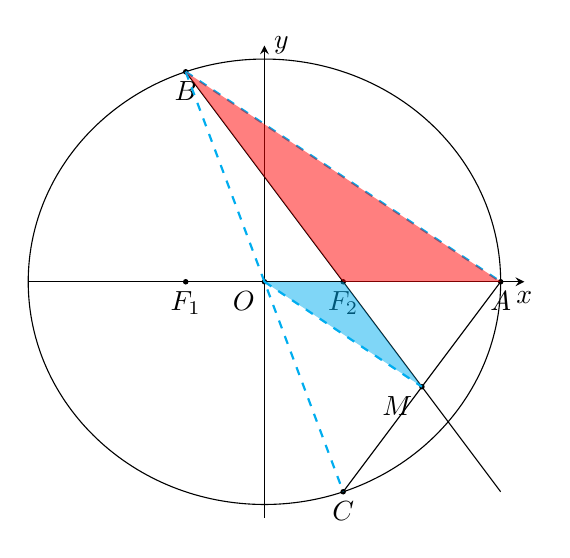
\begin{tikzpicture}
\pgfmathsetmacro\xx{3}
\pgfmathsetmacro\y{3}
\pgfmathsetmacro\a{3}
\pgfmathsetmacro\b{2*sqrt(2)}
\pgfmathsetmacro\c{sqrt(abs(\a^2-\b^2))}
\pgfmathsetmacro\px{-1}
\pgfmathsetmacro\py{sqrt(\b^2*(1-((\px)^2)/\a^2))}
\coordinate (O) at (0,0);
\coordinate (F1) at (-\c,0);
\coordinate (F2) at (\c,0);
\coordinate (B) at (\px,\py);
\coordinate (C) at ($(O)!-1!(B)$);
\coordinate (BF2) at ($(B)!2!(F2)$);
\coordinate (A) at (\a,0);
\draw[-stealth] (-\xx,0) -- (\xx+0.3,0) node [below] {$x$};
\draw[-stealth] (0,-\y) -- (0,\y) node [right] {$y$};
\draw[name path = a]  (B)--(BF2);
\draw[name path = b] (A) -- (C);
\draw(O) circle [x radius=\a,y radius=\b];
\fill [name intersections={of=a and b,by={M}}](M) circle (1pt) node [below left] {$M$};
\fill (O) node [below left] {$O$} circle (1pt);
\fill (F1) node [below] {$F_1$} circle (1pt);
\fill (F2) node [below] {$F_2$} circle (1pt);
\fill (A) node [below] {$A$} circle (1pt);
\fill (B) node [below] {$B$} circle (1pt);
\fill (C) node [below] {$C$} circle (1pt);
% \fill (F2) node [below] {$F_2$} circle (1pt);
\draw[cyan,dashed,thick] (O) -- (M) (B)--(C) (B)--(A);
\fill[cyan,opacity=0.5](O)--(M)--(F2)--cycle;
\fill[red,opacity=0.5](B)--(A)--(F2)--cycle;
\end{tikzpicture}
\end{document}